\documentclass[aspectratio=169]{beamer}

\usetheme{Madrid}
\usecolortheme{default}

\usepackage[T1]{fontenc}
\usepackage[utf8]{inputenc}
\usepackage{lmodern}
\usepackage{amsmath,amssymb}
\usepackage{graphicx}
\usepackage{booktabs}
\usepackage{tabularx}

\graphicspath{{figures/}{./}}

\title[AI-Ready HAPS--UAV Channel Model]{An AI-Ready Air-to-Ground Channel Model for Multi-Link HAPS--UAV Networks}
\author{Harsha Matadhikari \and Prof.~Sonali Garg \and Prof.~Abhishek Dixit}
\institute{Online PG Diploma in Advanced Communication Engineering with Quantum AI Integration \\ Indian Institute of Technology Delhi}
\date{}

\begin{document}

% ---------------------------------------------------------------
\begin{frame}
\titlepage
\end{frame}

% ---------------------------------------------------------------
\begin{frame}{Motivation}
\begin{itemize}
  \item A 3-HAPS equilateral-triangle constellation serves a ground footprint via
        \textbf{service} (2\,GHz), \textbf{backhaul} (38\,GHz), and two-hop
        \textbf{UAV relay} links.
  \item Co-channel interference from the other two HAPS makes SINR depend
        strongly on \emph{angular position}, not just distance -- an
        experimental finding of this paper, not prior knowledge.
  \item A simple rule-based policy cannot anticipate this, time-varying
        rain fades on the 38\,GHz backhaul, or battery depletion.
  \item \textbf{AI Ready Model:} a validated channel model, an LSTM rain
        forecaster, and a DQN agent that learns real-time user--platform
        association.
\end{itemize}

\vspace{4mm}
\begin{center}
\footnotesize
\textbf{Research flow:}\\[1mm]
\fbox{\parbox{0.27\textwidth}{\centering Attenuation \& channel models\\(FSPL, rain, fog, gas, scintillation, interference)}}
$\;\rightarrow\;$
\fbox{\parbox{0.22\textwidth}{\centering Baseline policies\\(random, max-SINR, max-throughput)}}
$\;\rightarrow\;$
\fbox{\parbox{0.27\textwidth}{\centering Learned policy\\(LSTM forecast + DQN) for\\platform selection}}
\end{center}
\end{frame}

% ---------------------------------------------------------------
\begin{frame}{System Topology and Channel Model}
\begin{columns}[T]
\begin{column}{0.5\textwidth}
\vspace{-11mm}
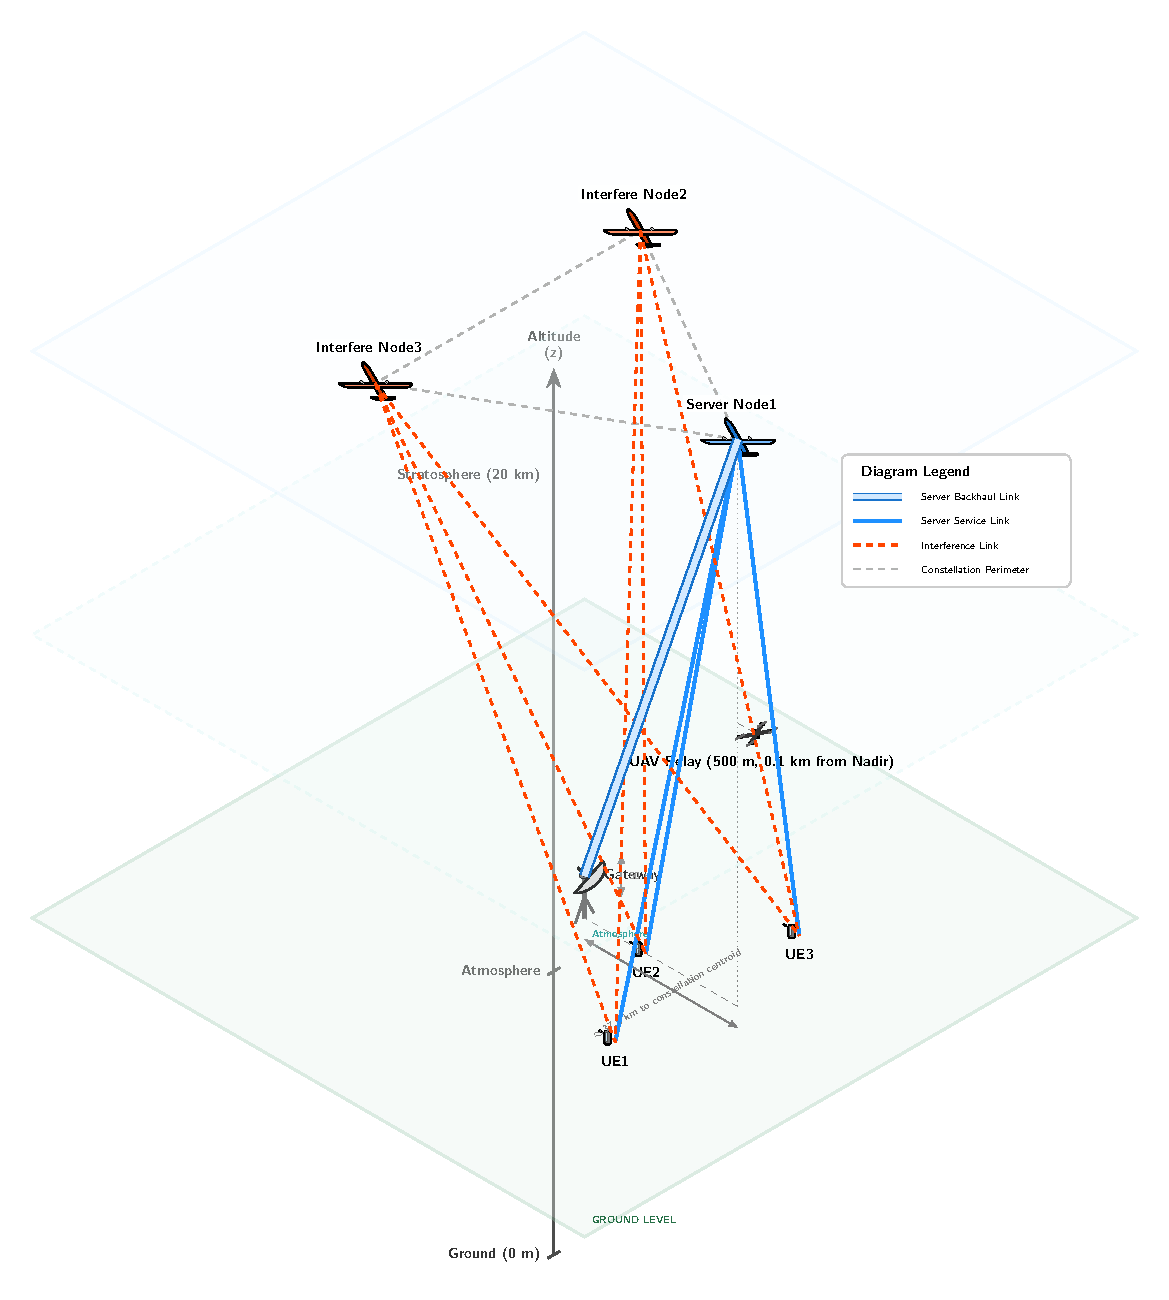
\includegraphics[width=\linewidth]{network_diagram_gw.pdf}
\end{column}
\begin{column}{0.5\textwidth}
\footnotesize
\textbf{Three link types:}
\begin{itemize}
  \item HAPS $\rightarrow$ UE (service, 2\,GHz)
  \item HAPS $\rightarrow$ Gateway (backhaul, 38\,GHz)
  \item HAPS $\rightarrow$ UAV $\rightarrow$ UE (relay; feeder hop at
        38\,GHz, UAV$\rightarrow$UE access hop at 2\,GHz)
\end{itemize}
\vspace{4mm}
\textbf{Channel model:}
\begin{itemize}
  \item Free-space path loss (all links)
  \item Building-blockage LoS/NLoS probability (2\,GHz UAV/HAPS access tier, Holis \& Pechac 2008)
  \item ITU-R rain, fog, gas, and scintillation losses (38\,GHz backhaul/feeder)
\end{itemize}
\vspace{2mm}
\textbf{Topology:} 3 HAPS (20\,km, 65\,km equilateral triangle), 1 static UAV relay (500\,m AGL, fixed 0.1\,km from the serving HAPS's own nadir), 1 gateway (50\,m AGL, fixed at the triangle's centroid instead).
\end{column}
\end{columns}
\end{frame}

% ---------------------------------------------------------------
\begin{frame}{Why 38\,GHz: Frequency Selection}
\begin{columns}[T]
\begin{column}{0.48\textwidth}
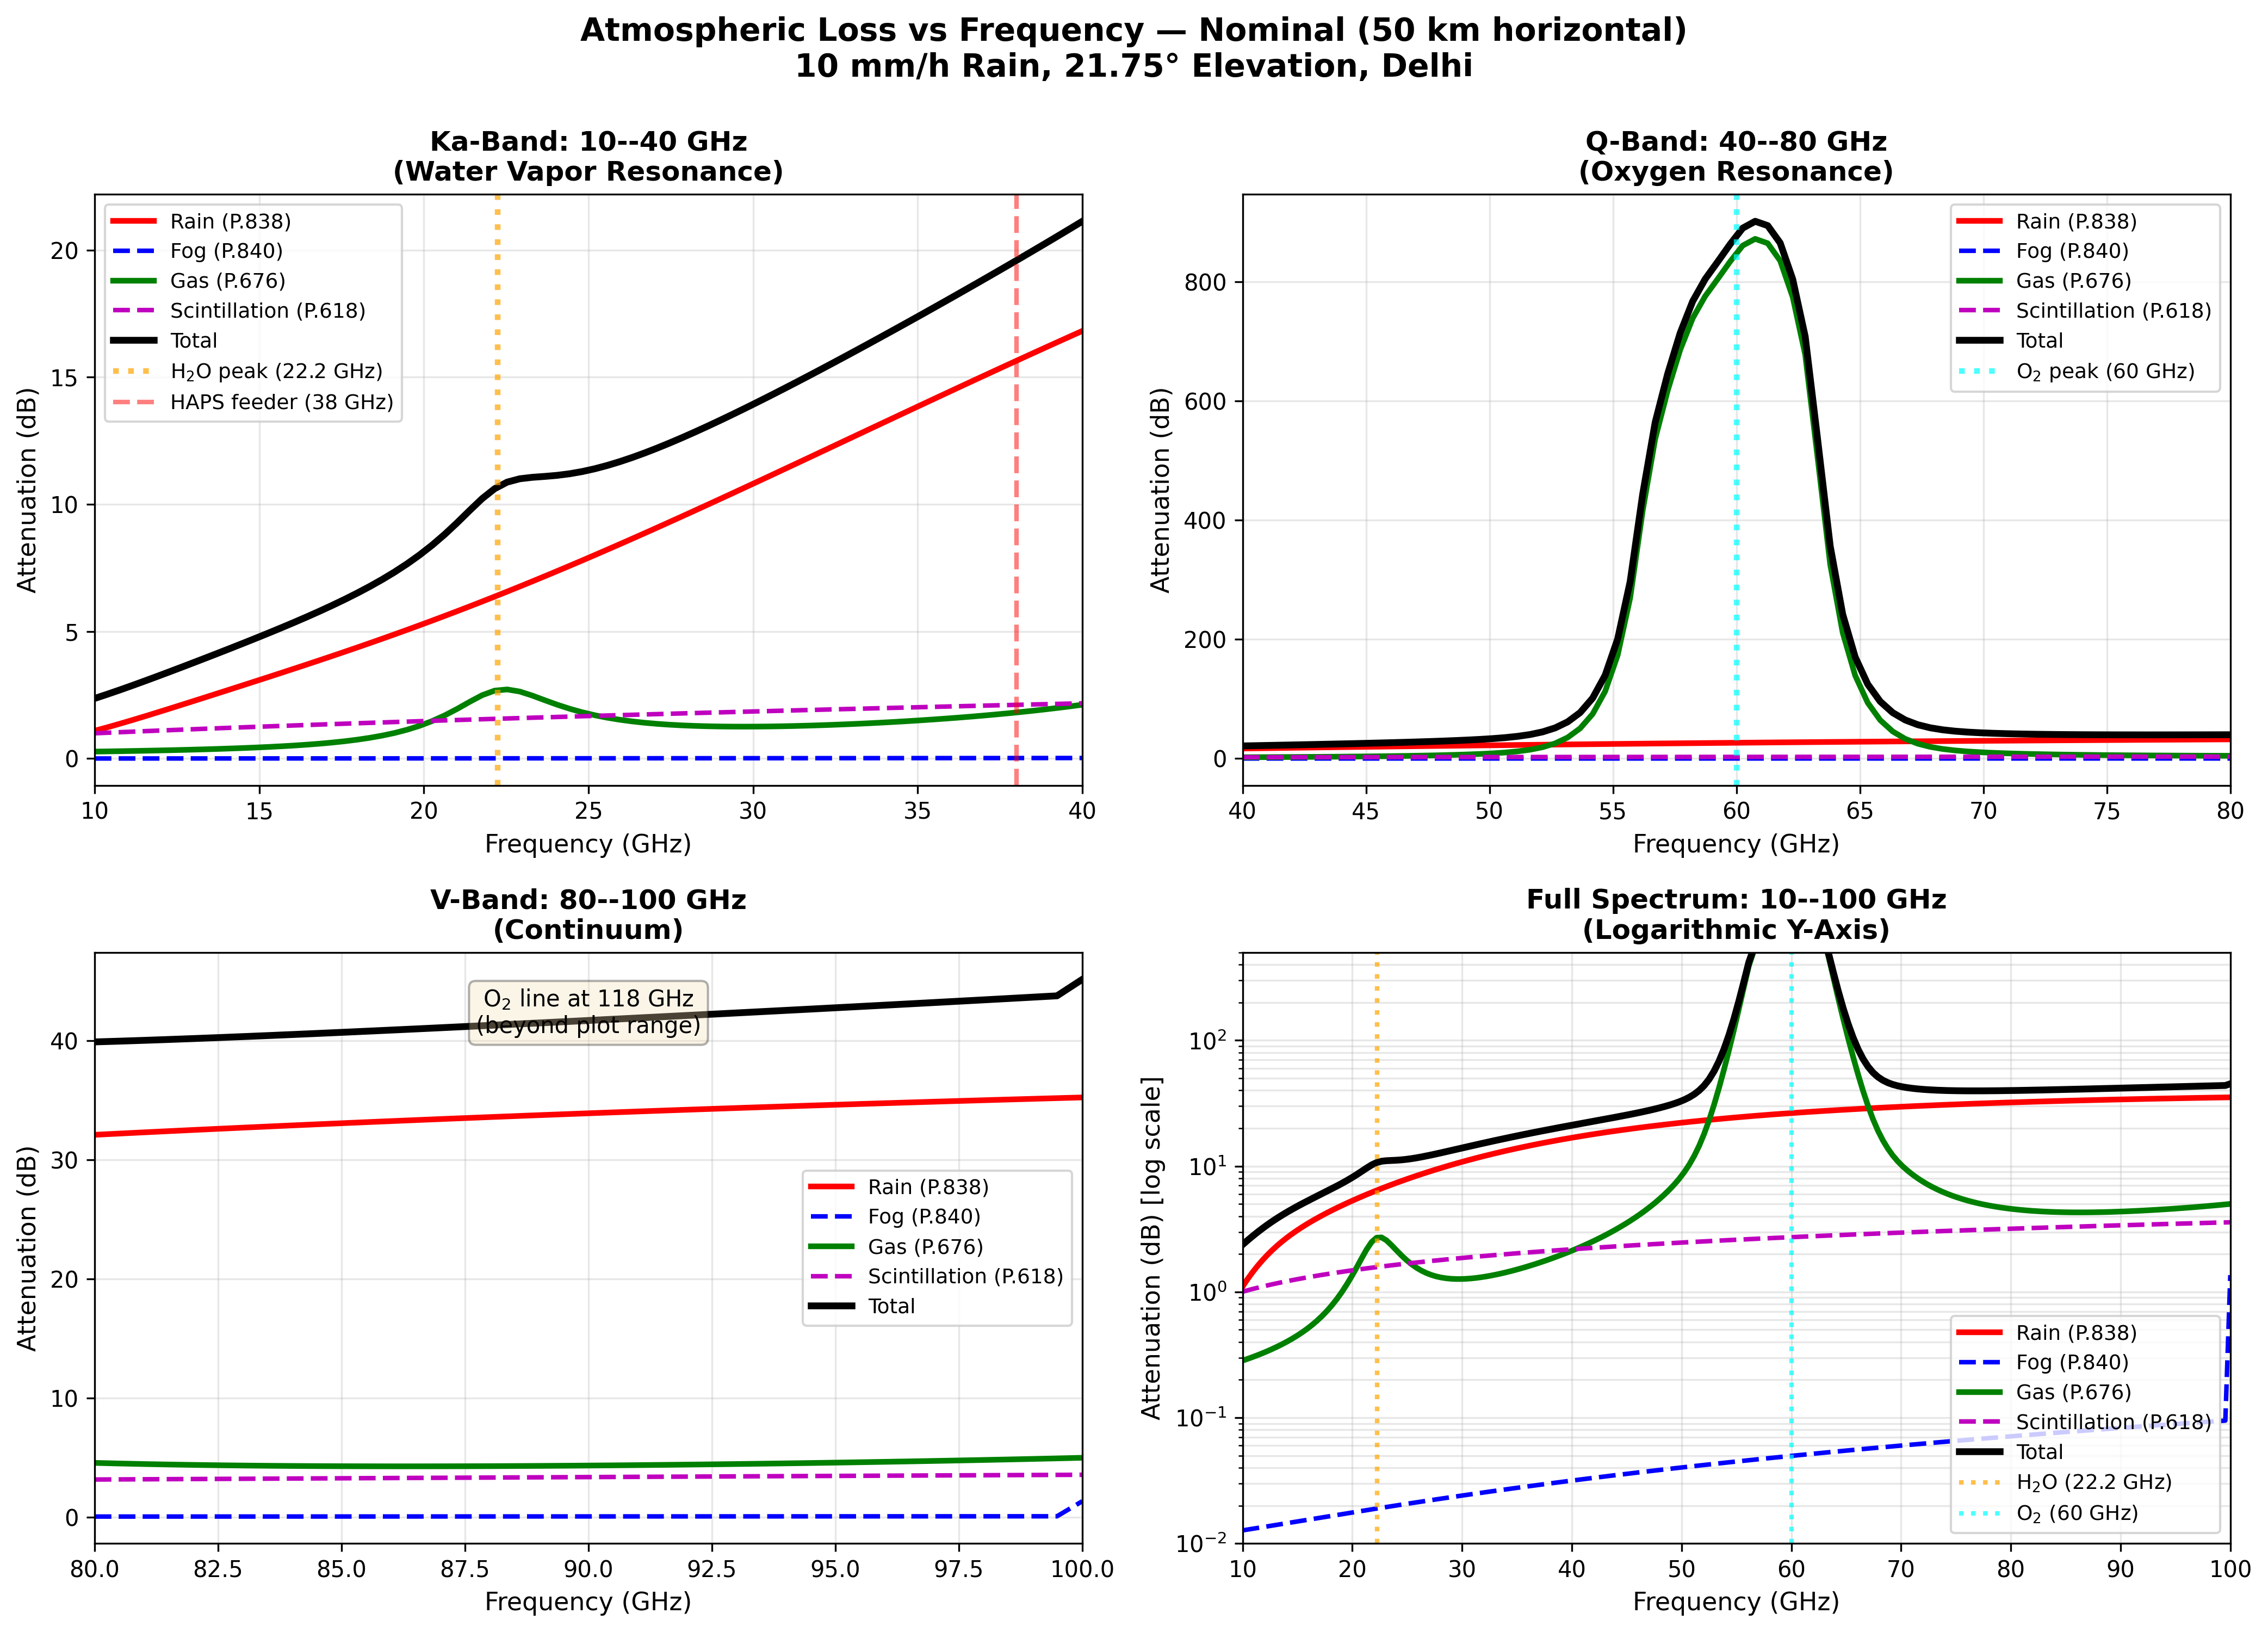
\includegraphics[width=\linewidth]{fig_atm_loss_nominal_frequency.png}
\end{column}
\begin{column}{0.52\textwidth}
\footnotesize
Atmospheric loss (rain, fog, gas) swept across the Ka/Q/V bands for
the Delhi gateway path, 10\,mm/h rain:
\begin{itemize}\setlength{\itemsep}{2pt}
  \item \textbf{Rain} (P.838/P.618) -- dominant term, grows roughly
        linearly with frequency; up to $\approx$19\,dB at 99.9\%
        availability ($R_{0.1}=15.7$\,mm/h).
  \item \textbf{Fog/cloud} (P.840) -- small except in dense fog;
        negligible below 10\,GHz.
  \item \textbf{Gas absorption} (P.676) -- two resonance peaks to
        avoid: H$_2$O at 22.2\,GHz, O$_2$ at 60\,GHz (there, total
        loss exceeds 800\,dB over 50\,km -- unusable).
\end{itemize}
\textbf{38\,GHz sits in the valley} between these peaks
($\approx$0.2--0.3\,dB/km clear-sky gas loss) -- this, not just
available bandwidth, is why it was chosen over a frequency closer to
either resonance.

\vspace{2mm}
\textbf{Backhaul budget:} $\approx$38\,dB clear-sky SINR comfortably
covers $\approx$19.4\,dB of rain+gas loss, leaving $\approx$18.6\,dB
margin at 99.9\,\% availability.
\end{column}
\end{columns}
\end{frame}

% ---------------------------------------------------------------
\begin{frame}{Angular Interference Sectors and Scintillation Fading}
\begin{columns}[T]
\begin{column}{0.48\textwidth}
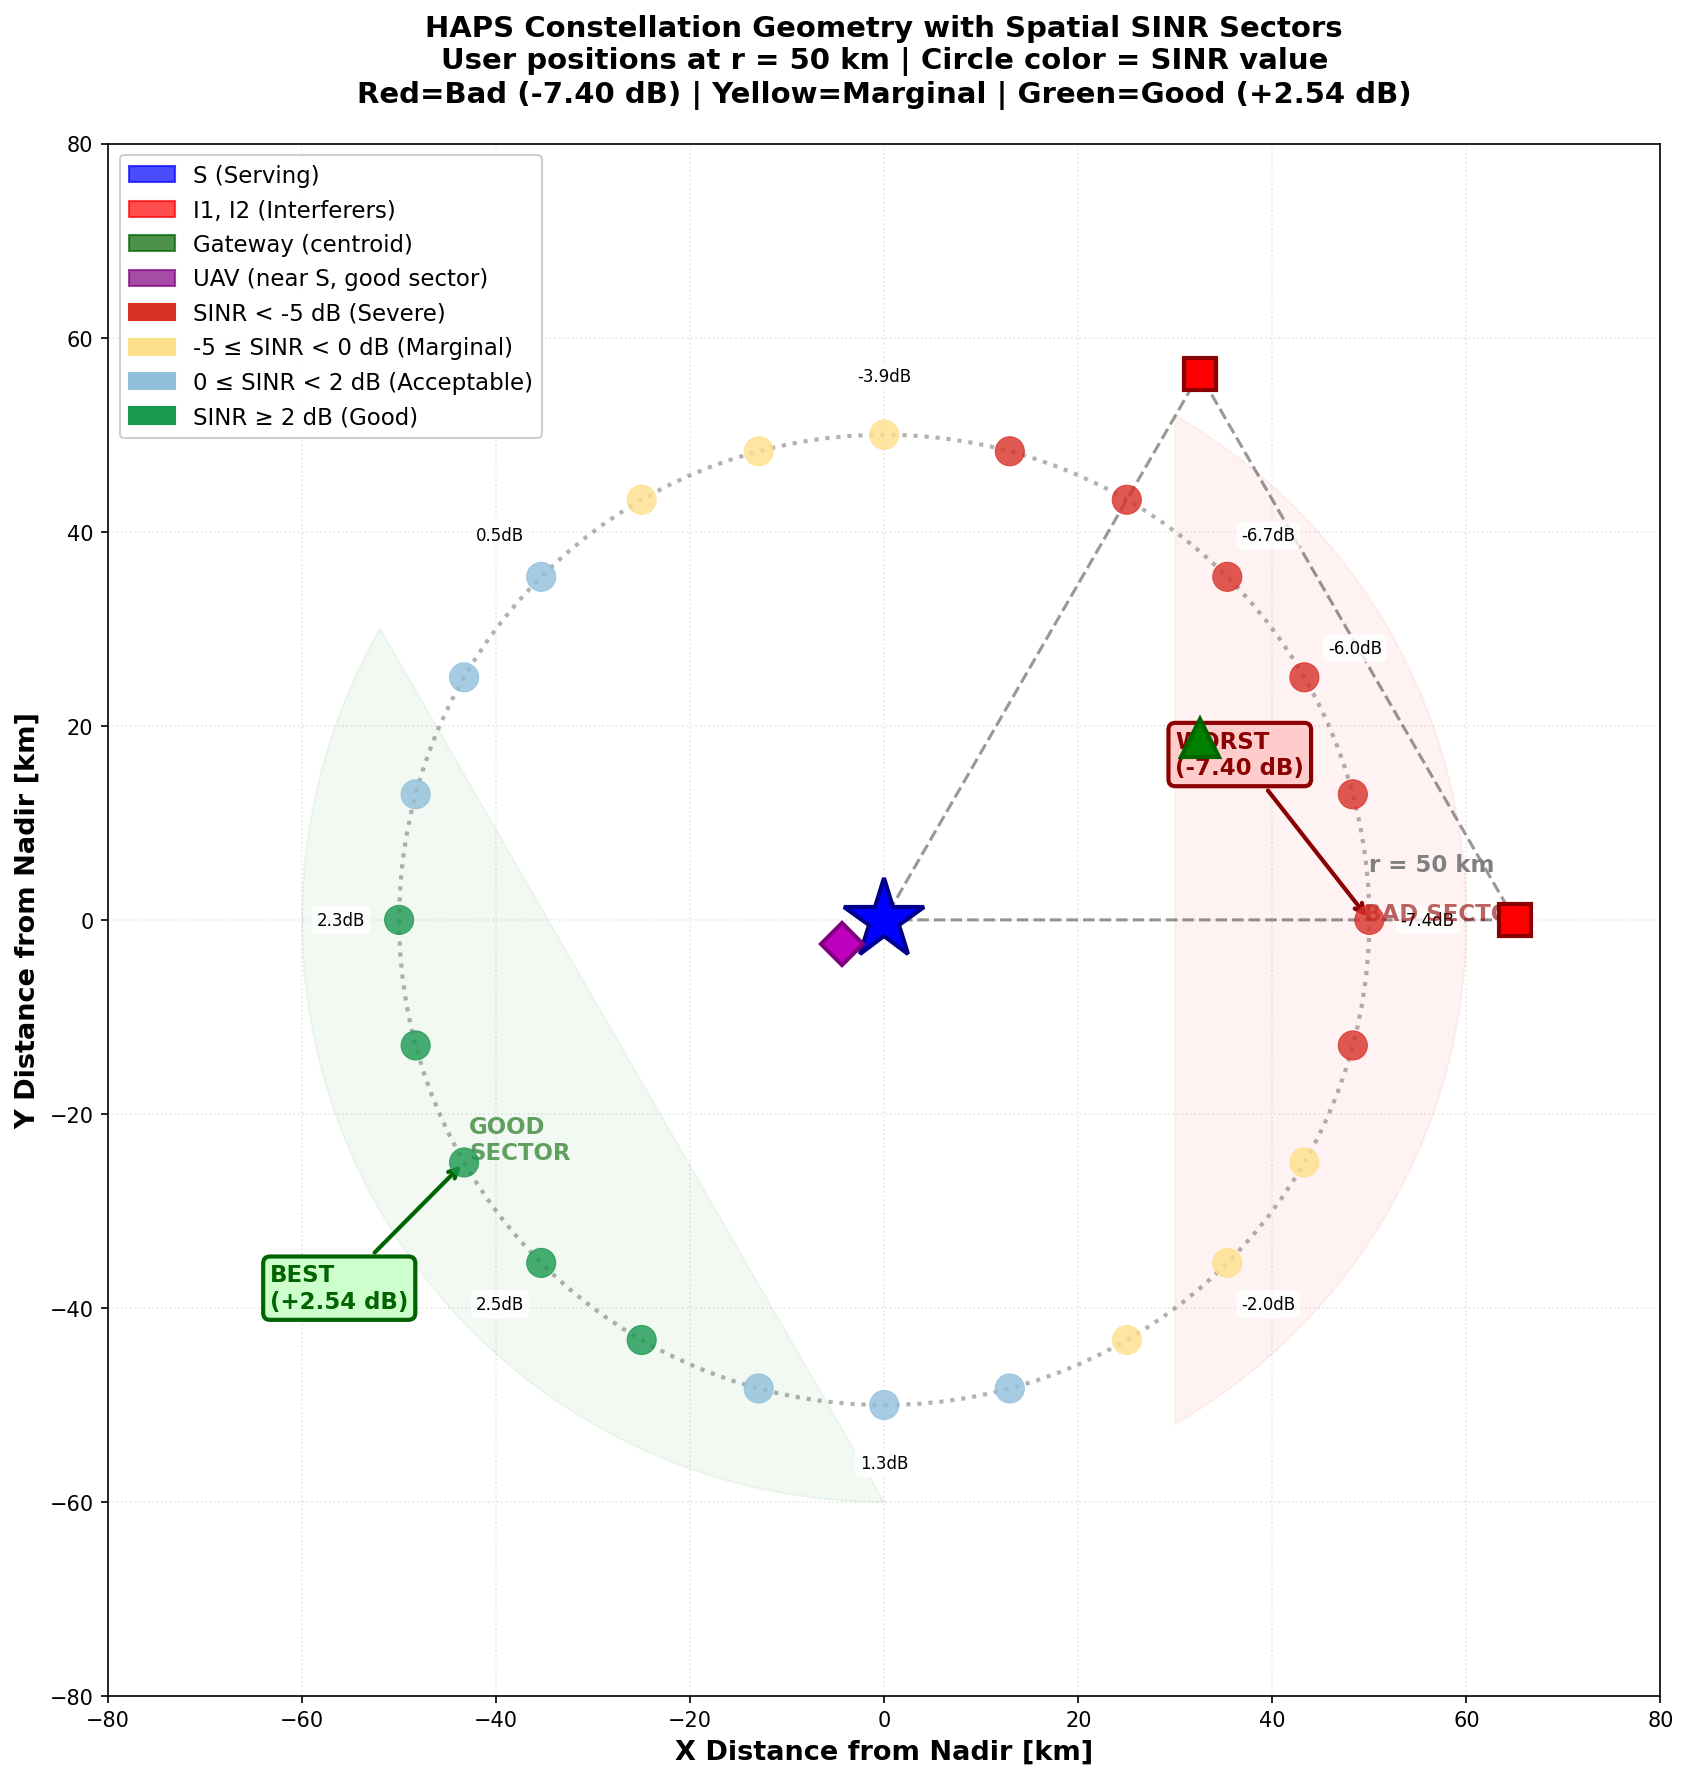
\includegraphics[width=\linewidth]{constellation_with_sectors.png}
\end{column}
\begin{column}{0.52\textwidth}
\footnotesize
\textbf{Angle-dependent SINR (sectors):} the 3-HAPS triangle creates a
good sector ($\approx$120\textdegree--290\textdegree, away from
interferers) and a bad sector ($\approx$330\textdegree--75\textdegree,
toward them) -- same radius, up to 9.94\,dB apart.

\vspace{2mm}
\textbf{Scintillation (ITU-R P.618):} rapid amplitude fluctuations
from tropospheric turbulence; grows with frequency, shrinks with
elevation. At 30\textdegree\ elevation, $p=0.01\%$: $\approx$0.49\,dB
at 38\,GHz vs.\ $\approx$0.09\,dB at 2.1\,GHz.

\vspace{2mm}
Favors positioning the UAV relay near nadir (higher elevation) when
feasible, especially for the HAPS--UAV feeder hop -- which also tends
to be away from the interferer-facing sector.

\vspace{2mm}
\scriptsize\textbf{Nuance:} each HAPS could simultaneously be a \emph{serving}
node (near-nadir, low-loss for its own users) and an \emph{interferer}
for the other two HAPS' users -- so this isn't a single clean
optimization across the constellation (future work, see Conclusion).
\end{column}
\end{columns}
\end{frame}

% ---------------------------------------------------------------
\begin{frame}{Spatial SINR Heterogeneity}
\begin{columns}[T]
\begin{column}{0.55\textwidth}
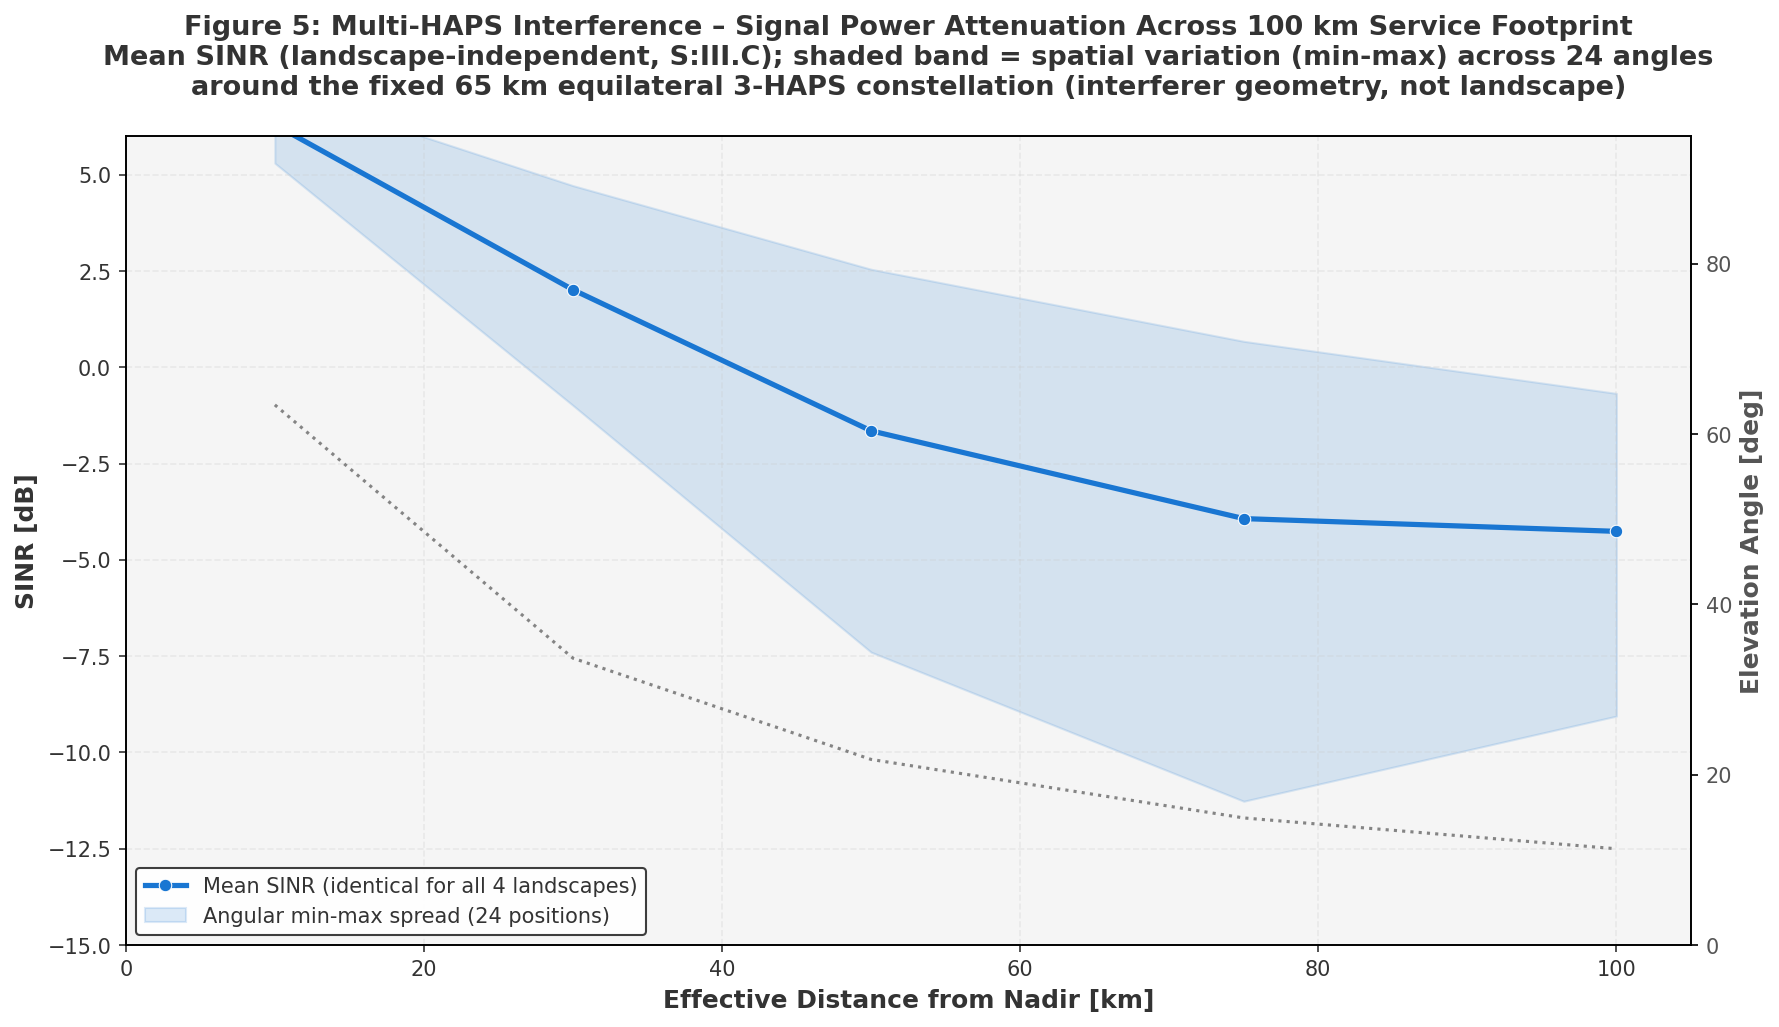
\includegraphics[width=\linewidth]{figure5_multi_haps_sinr_mean.png}
\end{column}
\begin{column}{0.45\textwidth}
\footnotesize
\begin{itemize}
  \item At a \textbf{fixed 50\,km radius}, SINR varies by
        \textbf{up to 9.94\,dB} depending on angular position relative to
        the two interfering HAPS.
  \item For comparison, simply \emph{doubling} the link distance only
        costs about 2--3\,dB -- so angular position affects SINR more
        than distance does.
  \item A simple ``always pick max-SINR'' rule cannot anticipate these
        angular patterns as a user moves or the constellation's
        geometry is reconsidered.
  \item Backhaul link stays noise-limited and essentially flat; the
        service link is the one exposed to this heterogeneity.
\end{itemize}
\end{column}
\end{columns}
\end{frame}

% ---------------------------------------------------------------
\begin{frame}{Relay Path Analysis (HAPS$\to$UAV$\to$UE)}
\begin{columns}[T]
\begin{column}{0.55\textwidth}
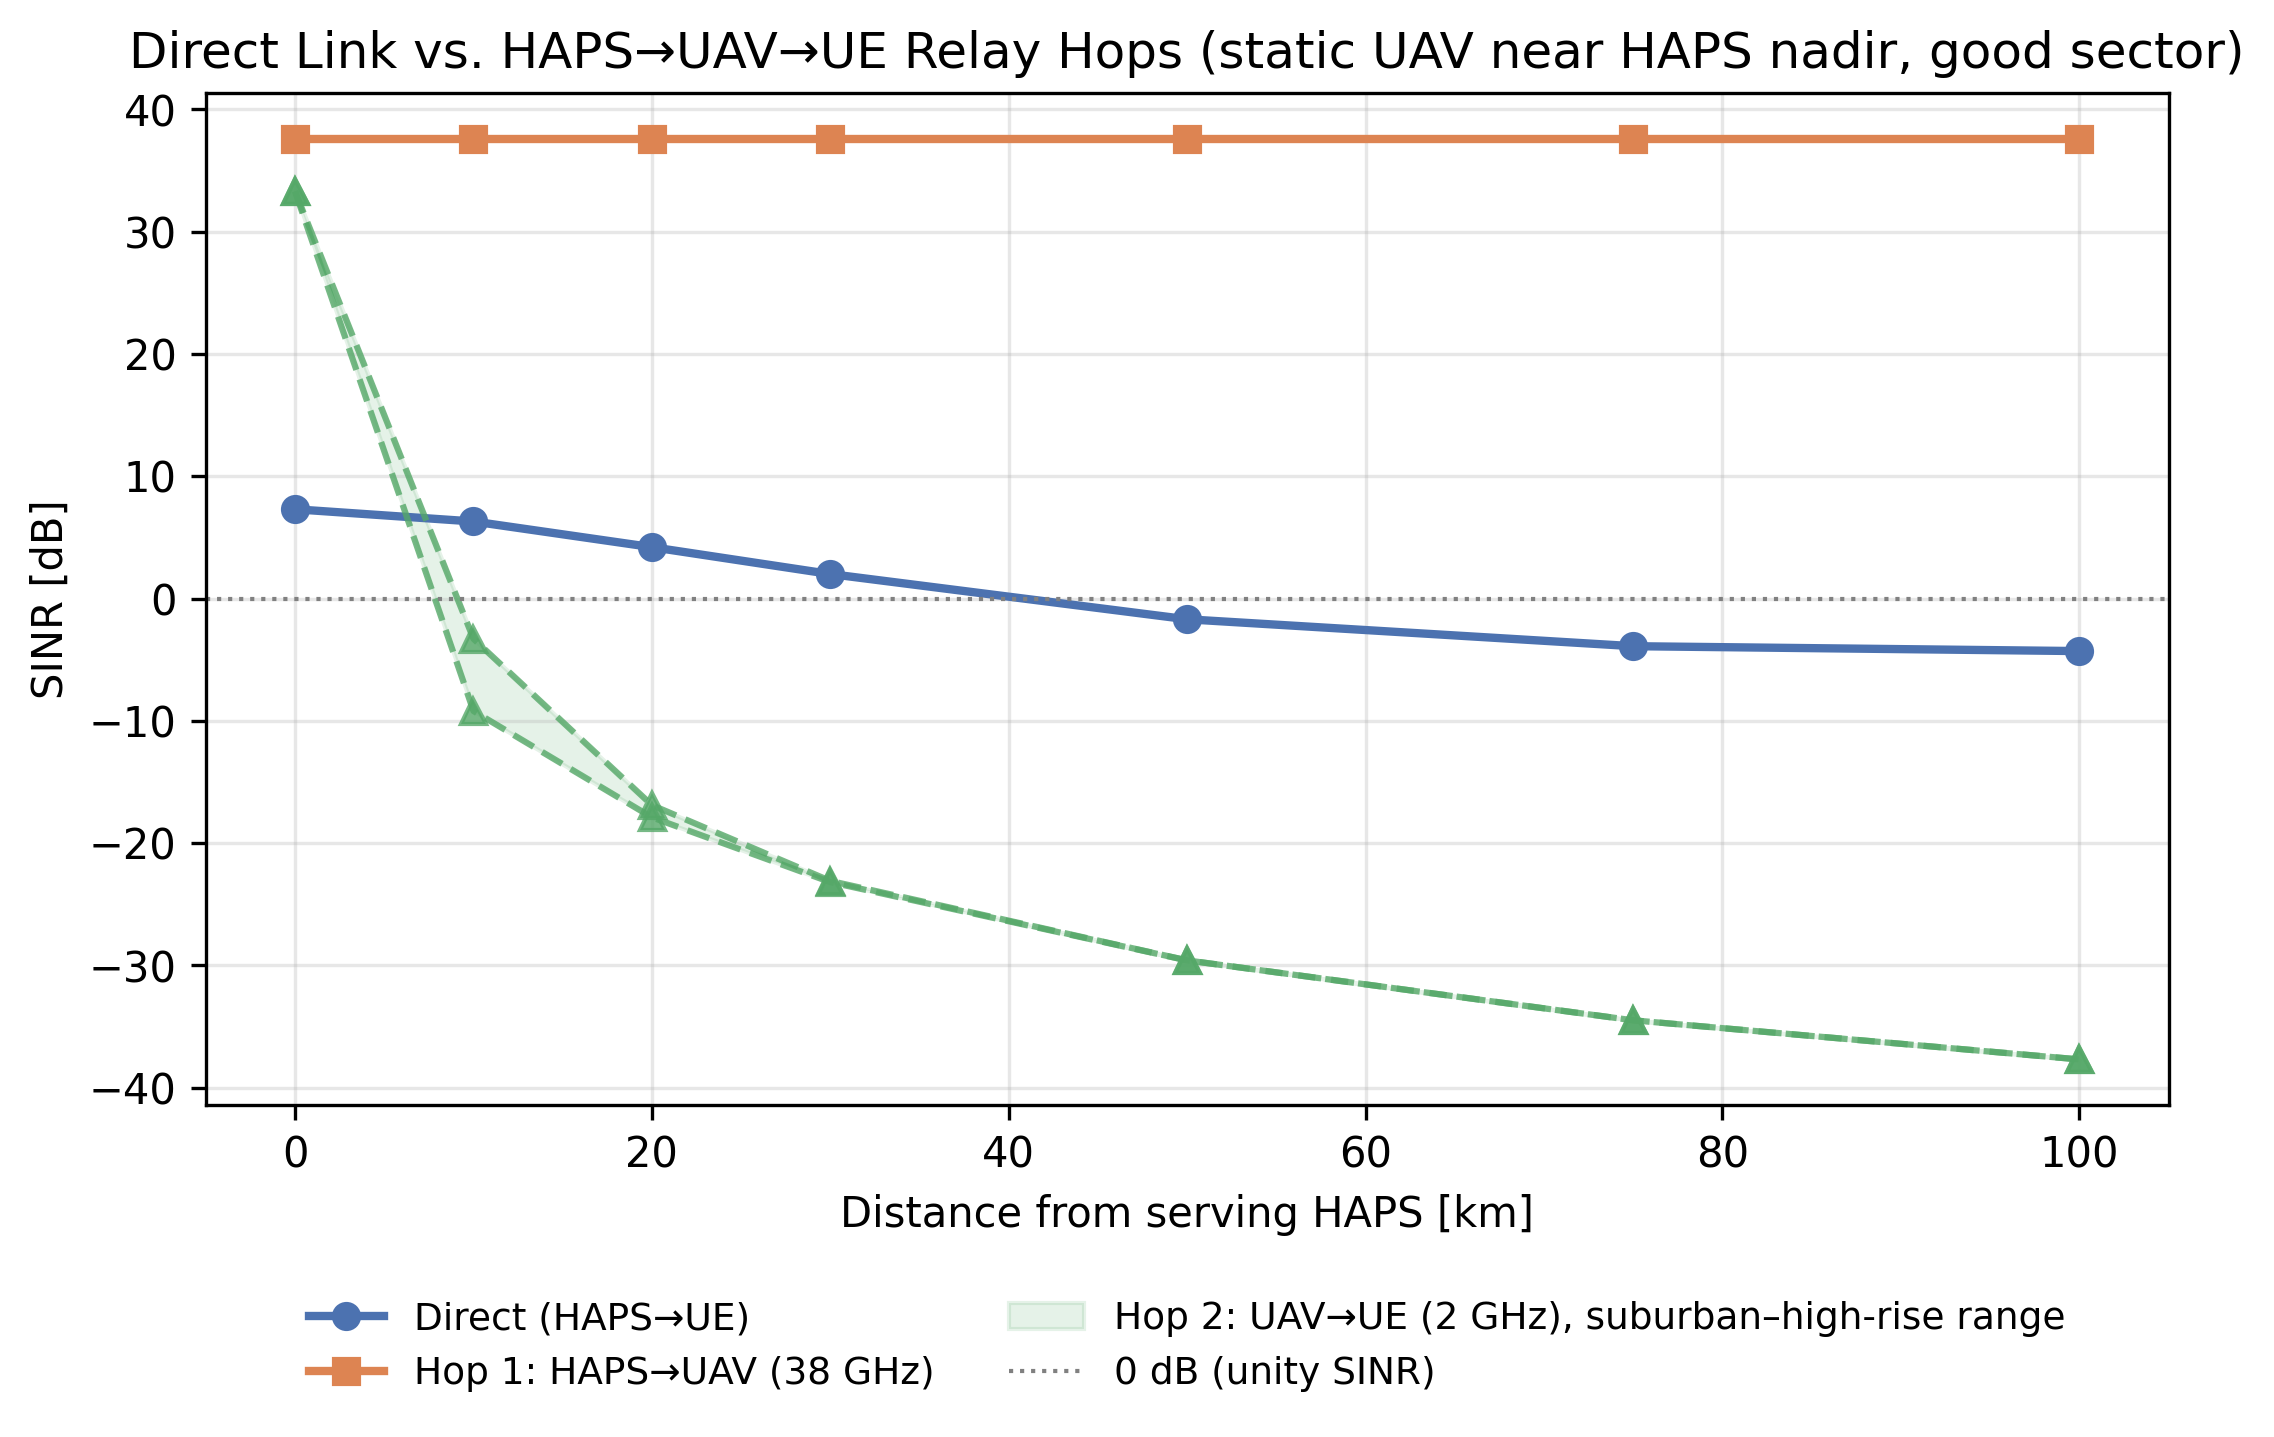
\includegraphics[width=\linewidth]{12_uav_relay_comparison.png}
\end{column}
\begin{column}{0.45\textwidth}
\footnotesize
\begin{itemize}
  \item Single static UAV, fixed 0.1\,km from the serving HAPS's own
        nadir (the Gateway occupies the centroid instead).
  \item \textbf{Feeder hop} (HAPS$\to$UAV, 38\,GHz): constant geometry
        by symmetry -- flat at $12.48$\,bits/s/Hz, $\approx$89.71\textdegree\
        elevation, for every HAPS.
  \item \textbf{Access hop} (UAV$\to$UE, 2\,GHz): collapses within a
        few km of the fixed UAV -- far faster than the direct link
        degrades with distance from a HAPS.
  \item Raw capacity: relay exceeds the direct link within
        $\approx$1--6\,km of the serving HAPS's own nadir, falling to
        $0.50$\,bits/s/Hz (direct: $\approx$2.5--2.6) at $R_\mathrm{eff}$.
  \item Contention: one HAPS's direct-link population ($100^2/3$,
        full footprint) outnumbers one UAV's relay population
        ($R_\mathrm{eff}^2$, its own disk) by $\approx$79:1 urban,
        31:1 suburban -- pure geometry, density cancels.
  \item Per-user share: relay beats direct \emph{everywhere} inside
        $R_\mathrm{eff}$ once this contention is priced in -- 15x at
        the urban disk's own edge, 6x suburban; more near the UAV.
        Beyond $R_\mathrm{eff}$, how far the advantage extends is open
        (needs real population-density data).
  \item Usable relay radius $\approx$6.5--10.3\,km $\Rightarrow$ still
        helps only users within one UAV's disk, not the 100\,km footprint.
  \item Full, gap-free 100\,km coverage would still need $\sim$200--270
        such UAVs placed away from each HAPS's own nadir (covering-number
        estimate, future work).
\end{itemize}
\end{column}
\end{columns}
\end{frame}

% ---------------------------------------------------------------
\begin{frame}{Motivation for Learning}
\footnotesize
A rule-based policy cannot account for three sources of variation this
paper's channel and platform models expose:
\begin{itemize}
  \item \textbf{Spatial SINR heterogeneity.} Angular position affects
        SINR more than distance -- a simple ``always pick max-SINR''
        rule cannot anticipate it as a user moves.
  \item \textbf{Time-varying weather.} Feeder-link rain attenuation
        must be anticipated before the hour it affects, since the
        association decision is made before that hour's rain is
        observed.
  \item \textbf{Battery depletion.} Each HAPS's state of charge
        depends on its load history, so load must be balanced across
        platforms over time to avoid over-draining any one HAPS.
\end{itemize}
A learned, real-time association policy can condition on all three
jointly.
\end{frame}

% ---------------------------------------------------------------
\begin{frame}{LSTM Rain-Attenuation Forecaster}
\begin{columns}[T]
\begin{column}{0.48\textwidth}
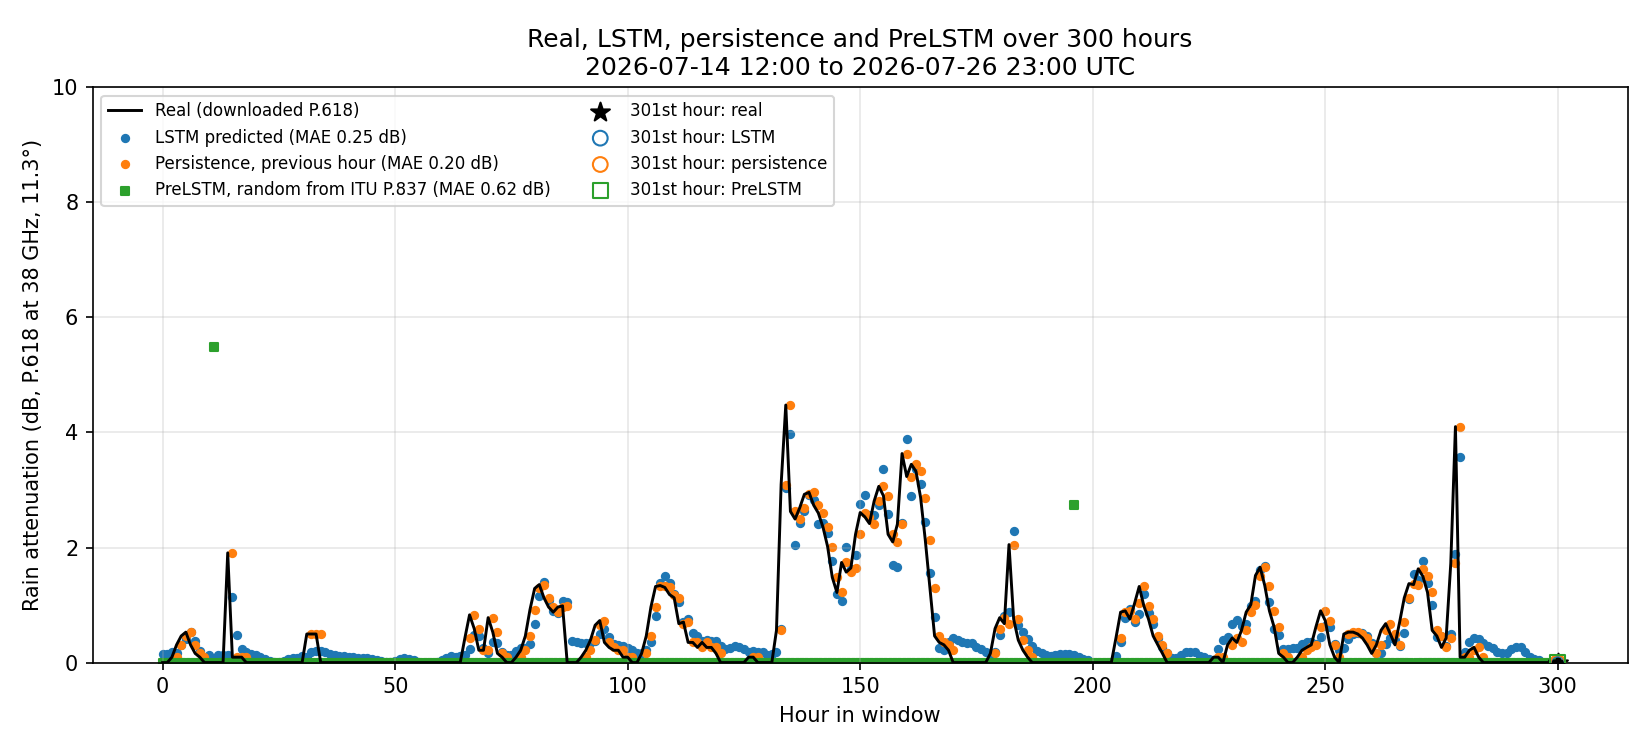
\includegraphics[width=\linewidth]{lstm_forecast_2026.png}
\vspace{2mm}
\footnotesize
\begin{itemize}\setlength{\itemsep}{2pt}
  \item DQN must decide at hour $t$ \emph{before} that hour's rain is
        observed $\Rightarrow$ needs a forecast.
  \item Early-stopped on held-out 2025 validation RMSE to avoid
        overfitting; 2026 untouched until final evaluation.
  \item Evaluated \textbf{out-of-sample}: 2026 forecasts from a model
        trained only on 2023--2025 data.
\end{itemize}
\end{column}
\begin{column}{0.52\textwidth}
\footnotesize
\begin{itemize}\setlength{\itemsep}{2pt}
  \item LSTM predicts feeder (38\,GHz) rain attenuation up to
        \textbf{six hours ahead} from NASA POWER / METAR / ERA5
        weather history for Delhi.
  \item Lower RMSE than persistence at every horizon except
        $+1$\,h, where persistence is slightly better; all six
        horizons feed the DQN's state.
\end{itemize}

\vspace{2mm}
{\scriptsize\setlength{\tabcolsep}{3pt}
\begin{tabularx}{\linewidth}{|>{\centering\arraybackslash}X|>{\centering\arraybackslash}X|>{\centering\arraybackslash}X|}
\hline
\textbf{Horizon} & \textbf{LSTM RMSE} & \textbf{Persist.\ RMSE} \\
\hline
$+1$\,h & $0.54$ & $\mathbf{0.53}$ \\
\hline
$+3$\,h & $\mathbf{0.80}$ & $0.90$ \\
\hline
$+6$\,h & $\mathbf{0.92}$ & $1.17$ \\
\hline
\end{tabularx}}
\end{column}
\end{columns}
\end{frame}

% ---------------------------------------------------------------
\begin{frame}{DQN Association Agent: Problem Formulation}
\footnotesize
\textbf{Per-user MDP} -- each user independently chooses a platform; network
reward is computed after all assignments. With a single static UAV, which
HAPS feeds its feeder hop is folded into the same per-user action set.
\vspace{2mm}

\begin{columns}[T]
\begin{column}{0.48\textwidth}
\begin{itemize}\setlength{\itemsep}{3pt}
  \item \textbf{State (21-dim):} SINR to each platform, distance,
        battery SoC, UAV-relay capacity, rainfall, visibility,
        time-of-day, six LSTM rain forecasts.
  \item \textbf{Action:} $a_k \in \{0,\dots,5\}$ -- direct link to
        HAPS1--3, or relay through the UAV served by HAPS1--3.
\end{itemize}
\end{column}
\begin{column}{0.52\textwidth}
\begin{itemize}\setlength{\itemsep}{3pt}
  \item \textbf{Reward:} rain-derated throughput + fairness (Jain
        index) $-$ energy cost $-$ outage/degraded-service penalties
        $-$ low-battery penalty.
\end{itemize}
\vspace{2mm}
\begin{itemize}\setlength{\itemsep}{3pt}
  \item Custom Deep Q-Network implemented directly in PyTorch
        (\texttt{torch}/\texttt{torch.nn}).
  \item Trained on 2400 rolling 24-hour episodes (400 real 2024
        episodes, cycled six times); evaluated on 50 held-out 2025
        days across ten experiments (random seeds).
\end{itemize}
\end{column}
\end{columns}
\end{frame}

% ---------------------------------------------------------------
\begin{frame}{Results: Policy Comparison}
\footnotesize
\begin{table}
\centering
\begin{tabularx}{\linewidth}{|>{\raggedright\arraybackslash}X|>{\centering\arraybackslash}X|>{\centering\arraybackslash}X|>{\centering\arraybackslash}X|}
\hline
\textbf{Policy} & \textbf{Reward/step} & \textbf{Jain} & \textbf{Outage /50} \\
\hline
Random (six actions) & $-92.2\,(1.4)$ & $0.255\,(0.011)$ & $41.6\,(0.3)$ \\
\hline
Max-SINR (direct only) & $-14.5\,(1.7)$ & $\mathbf{0.558}\,(0.013)$ & $\mathbf{0.8}\,(0.2)$ \\
\hline
Max-throughput (six actions) & $\mathbf{-14.6}\,(1.7)$ & $0.241\,(0.039)$ & $\mathbf{0.8}\,(0.2)$ \\
\hline
LSTM + DQN & $-15.1\,(1.7)$ & $0.351\,(0.112)$ & $1.2\,(0.2)$ \\
\hline
\end{tabularx}
\end{table}
\begin{itemize}
  \item Mean $\pm$ std.\ dev.\ over ten experiments, 50 held-out 2025 days.
  \item LSTM+DQN is behind both rule-based baselines on reward and
        outage, and behind max-SINR on fairness, but \textbf{fairer
        than max-throughput} (Jain $0.351$ vs.\ $0.241$, 8/10 seeds).
  \item Max-SINR and max-throughput both need continuous, perfect,
        zero-latency measurement of every platform's SINR or capacity
        from every UE -- an idealized assumption, not something a
        real UE can actually provide. Loading all crowded users onto
        max-throughput's single best option is also why its own
        fairness collapses ($0.241$) once contention is modelled.
  \item The DQN uses only its own locally available state and allows
        dynamic switching of links based on practical,
        learned-from-past-data behaviour -- the only one of the three
        that is actually deployable, and the only one that retains
        and uses the relay path.
\end{itemize}
\end{frame}

% ---------------------------------------------------------------
\begin{frame}{Results: Stability Across Experiments}
\begin{columns}[T]
\begin{column}{0.48\textwidth}
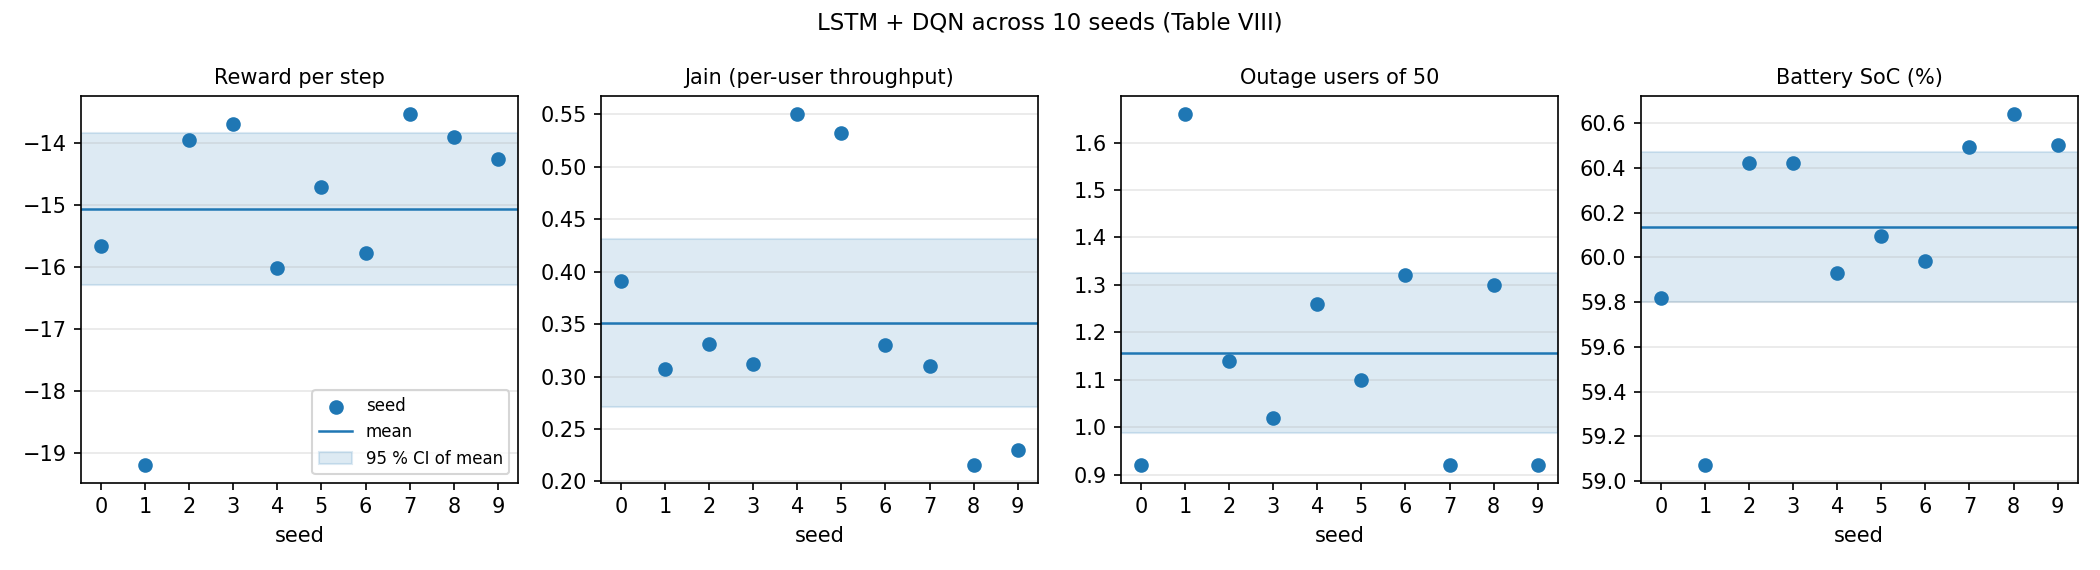
\includegraphics[width=\linewidth]{seed_stats.png}
\vspace{2mm}
\scriptsize
\textbf{LSTM + DQN, ten independent seeds} (dot = one training run;
line = mean; band = 95\% CI \emph{of the mean}):
\begin{itemize}\setlength{\itemsep}{0pt}
  \item Reward/step: $-15.07 \pm 1.71$ \\ (95\% CI $[-16.30, -13.85]$)
  \item Jain fairness: $0.351 \pm 0.112$
  \item Outage: $1.16 \pm 0.24$ of 50 users
  \item Battery SoC: $60.14 \pm 0.47\,\%$
\end{itemize}
\end{column}
\begin{column}{0.52\textwidth}
\scriptsize
\textbf{CI vs.\ spread:} the shaded band is \emph{not} ``most runs land
here'' -- it narrows with more seeds and reflects precision of the
estimated mean, not run-to-run spread.

\vspace{2mm}
\textbf{Takeaway:} the tight spread across all ten seeds shows the
policy is \textbf{reliably learned} to this level, not a lucky or
unlucky single run -- consistency, not the reward level itself, is
what this figure demonstrates.
\end{column}
\end{columns}
\end{frame}

% ---------------------------------------------------------------
\begin{frame}{Results: Statistical Significance}
\begin{columns}[T]
\begin{column}{0.42\textwidth}
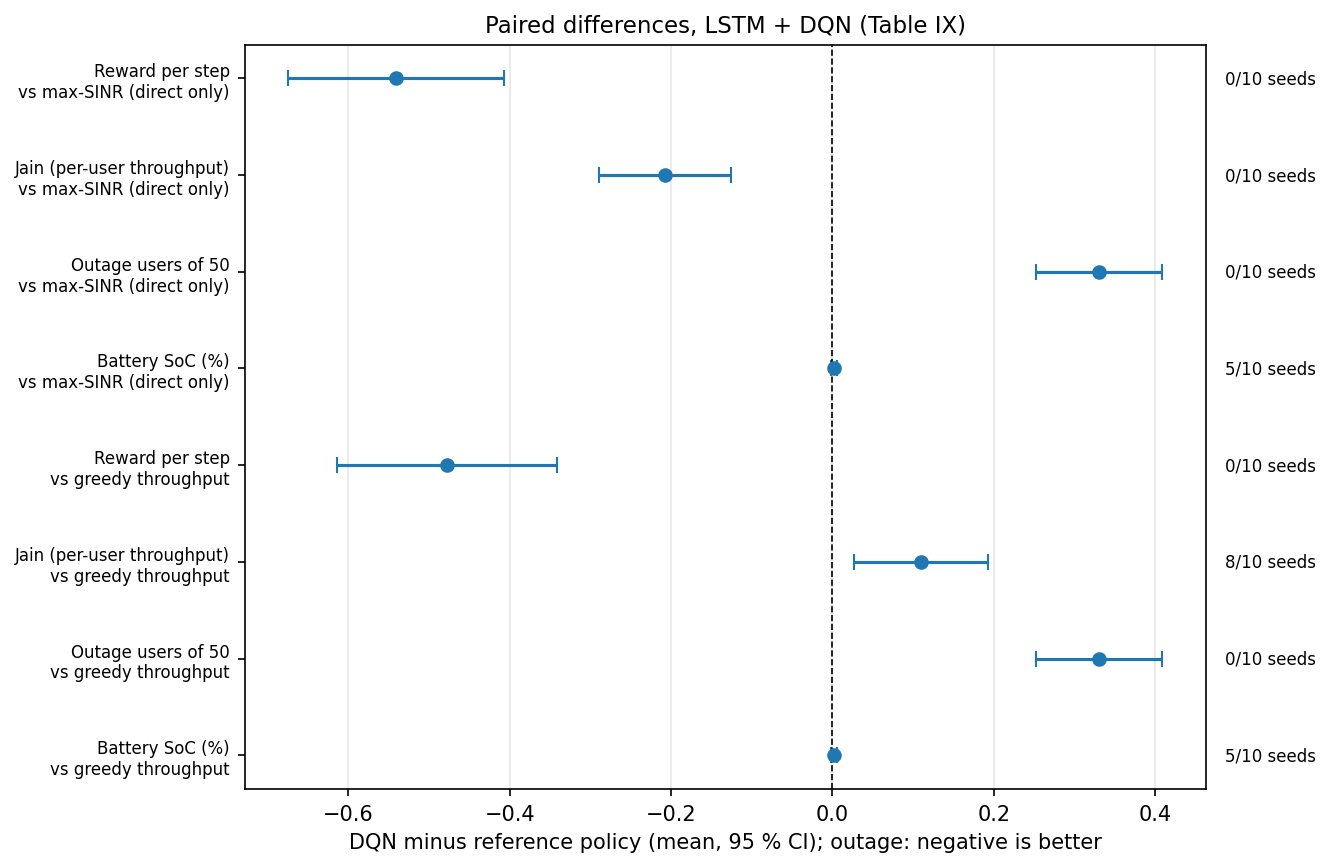
\includegraphics[width=\linewidth]{paired_forest.png}
\end{column}
\begin{column}{0.58\textwidth}
\scriptsize
Paired differences, LSTM+DQN minus baseline (per experiment, 50 days
each, ten seeds). Whiskers crossing 0 = not significant.

\vspace{1mm}
\textbf{vs.\ Max-SINR:}
\begin{itemize}\setlength{\itemsep}{0pt}
  \item Reward: $-0.54$ ($p<0.0001$, $0/10$ seeds favoring DQN)
  \item Jain: $-0.207$ ($p=0.0003$, $0/10$)
  \item Outage: $+0.33$, i.e.\ worse ($p<0.0001$, $0/10$)
  \item Battery SoC: $\approx 0$ ($p=0.33$, tie)
\end{itemize}

\vspace{1mm}
\textbf{vs.\ Max-throughput:}
\begin{itemize}\setlength{\itemsep}{0pt}
  \item Reward: $-0.48$ ($p<0.0001$, $0/10$)
  \item Jain: $\mathbf{+0.110}$, i.e.\ \textbf{fairer} ($p=0.0153$, $8/10$)
  \item Outage: $+0.33$, i.e.\ worse ($p<0.0001$, $0/10$)
  \item Battery SoC: $\approx 0$ ($p=0.33$, tie)
\end{itemize}

\vspace{1mm}
\textbf{Takeaway:} the DQN loses to both rule-based policies on
reward and outage on every seed, and to max-SINR on fairness on
every seed, but is \textbf{fairer than max-throughput} on 8/10 seeds
-- and still uniquely uses the relay path as a targeted fallback.
\end{column}
\end{columns}
\end{frame}

% ---------------------------------------------------------------
\begin{frame}{Does the Rain Forecast Help the DQN Itself?}
\footnotesize
A forecast ablation (\texttt{lstm} vs.\ \texttt{none}, rain-forecast
features removed, vs.\ \texttt{oracle}, true future attenuation given)
finds all three statistically indistinguishable on reward, fairness,
and outage ($p>0.1$) -- and it stays null after two further tests:
\begin{itemize}
  \item \textbf{Gave the UAV feeder its own rain fade.} Previously
        unmodelled; its near-zenith path actually fades \emph{more}
        than the backhaul's at most rain rates. Still null.
  \item \textbf{Added a per-user switching-cost penalty.} Tests
        whether reacting late (vs.\ anticipating) is the missing
        friction. Still null -- with one UAV, there is no
        penalty-free alternative to pre-emptively move traffic to.
  \item \textbf{Why:} this MDP lets every user react to the current
        hour's rain for free -- raw rain rate is already a state
        feature regardless of the forecast. A forecast only pays off
        when reacting late costs something real.
  \item \textbf{Where it would matter:} a fleet, where a fade over
        one HAPS squeezes every UAV feeding off it at once --
        forcing a synchronized surge of handovers unless the policy
        can see it coming and stagger them.
\end{itemize}

\vspace{2mm}
\textbf{Takeaway:} rain does not impact runs on this geometry -- the
2\,GHz access link and the margin-supported 38\,GHz feeder link both
absorb it without needing to anticipate it. The forecaster's behaviour
against persistence is nonetheless a useful input for more complex
geometries where margins no longer absorb rain's losses.
\end{frame}

% ---------------------------------------------------------------
\begin{frame}{Conclusion and Future Work}
\scriptsize
\textbf{Backhaul.} Noise-limited, largely unaffected by constellation
geometry, and largely insulated from rain by its design margin.
\quad
\textbf{Service.} Spatial SINR heterogeneity (up to 9.94\,dB at fixed
50\,km) dominates quality; cannot multiplex simultaneous users, so
cannot scale to replace the relay.
\quad
\textbf{Relay.} Access hop collapses within a few km; but once
contention is modelled (one HAPS's direct-link crowd is $\approx$79x
a UAV's relay crowd, by geometry alone), relay beats direct
\emph{everywhere} inside its own disk. One static UAV still only
covers that one disk ($\approx$6.5\,km radius; $\sim$200--270 UAVs
for full coverage).
\quad
\textbf{Learned association.} Measurably, if narrowly, behind both
rule-based baselines on reward ($p<0.0001$), but using only its own
locally available state, not the continuous, perfect, zero-latency
global measurement the baselines require -- the only one of the three
that is actually deployable.

\vspace{2mm}
\textbf{Roadmap for future work:}
\begin{itemize}\setlength{\itemsep}{0pt}
  \item \emph{Model multiple UAVs:} positioning for best SINR,
        UAV$\to$HAPS association for $N$ UAVs/$M$ HAPS, and a
        UAV-to-UAV interference term plus relative motion of HAPS
        and UAVs.
  \item \emph{LSTM and DQN improvements:} rain forecasting may help
        once a fleet of UAVs changes the action space; other
        impairments (fog, scintillation, gas) are not yet analysed as
        time series; the DQN's feeder-HAPS choice should condition on
        a per-UAV, physically grounded feeder-channel state rather
        than the single global mean user state used here.
  \item \emph{Dynamic topology and geometry:} changing HAPS roles
        (serving vs.\ interfering) and jointly optimizing positioning
        across both; beamforming between HAPS and gateway.
\end{itemize}

\vspace{2mm}
\centering \large Thank you -- Questions?
\end{frame}

\end{document}
